Tritium is the only radioactive isotope of hydrogen. It was first time produced in $1934$ from neutron capture of deuterium by Ernest Rutherford, Mark Oliphant and Paul Harteck \cite{TritiumDiscovery} and it was first time isolated in 1939 by Luis Walter Alvarez and Robert Cornog \cite{TritiumIsolate}, who checked that tritium is a radiactive element. 

Tritium can be found in the environment since it is normally produced through the interaction of cosmics rays and gaseous elements of the upper atmosphere like nitrogen ($\ce{^{14}N}(\ce{n},\ce{^{3}H})\ce{^{12}C}$) \cite{TritiumHandling} and oxigen ($\ce{^{16}O}(\ce{n},\ce{^{3}H})\ce{^{14}N}$) \cite{OxigenTritium}. Then tritium becomes water (\ce{HTO}) and reaches the earth's surface as rain with an estimated produccion rate of $4\cdot 10^6 ~\curie/$yr \newline ($1.48 \cdot 10^8 ~\giga\becquerel/$yr) \cite{CommonEmissionTritium} \cite{TritiumHandling} . 

Tritium can be produced artificially in the environment from many different anthropogenic origins. There are a big amount of tritium which was produced on militar nuclear test explosions between 1945 and 1975, whose estimed produccion rate is $8 \cdot 10^9~\curie$ ($2.96 \cdot 10^11~\giga\becquerel$) and a part of that still remain. It was mainly produced from the nuclear reactions $\ce{^{14}N}(\ce{n},\ce{^{3}H})\ce{^{12}C}$ and $\ce{^{2}H}(\ce{n},\gamma)\ce{^{3}H}$. Tritium can be also produced by commercial producers of radioluminicent and neutron generator devices ($1 \cdot 10^6$ $~\curie/$yr), nuclear power and defense industries (less than $2 \cdot 10^6~\curie/$yr), several research facilities and nuclear reactor operation ($2 \cdot 10^6 \curie/\giga\watt$yr), whose main production channels are \cite{CommonEmissionTritium} \cite{TritiumHandling}:

\begin{equation}
\ce{^{2}_{1}H}(\ce{n},\gamma)\ce{^{3}_{1}H} \qquad \sigma_{th}= 5.2 \cdot{} 10^{-4}~\barn  ~~~\cite{CommonEmissionTritium}
\label{capneuH2}
\end{equation}

\begin{equation}
\ce{^{3}_{2}He}(\ce{n},\ce{p})\ce{^{3}_{1}H} \qquad \sigma_{th}= 5330~\barn ~~~\cite{CommonEmissionTritium}
\label{capneuHe3}
\end{equation}

\begin{equation}
\ce{^{6}_{3}Li}(\ce{n},\alpha)\ce{^{3}_{1}H} \qquad \sigma_{th}= 940~\barn ~~~\cite{CommonEmissionTritium}
\label{capneuLi6}
\end{equation}

%%\begin{equation}
%%\ce{^{7}_{3}Li}(\ce{n},\alpha)\ce{^{3}_{1}He} + \ce{n} ~~~\cite{CommonEmissionTritium}
%%\label{capneuLi7}
%%\end{equation}

\begin{equation}
\ce{^{10}_{5}B}(\ce{n},2\alpha)\ce{^{3}_{1}H} \qquad \sigma_{th}= 3835~\barn ~~~\cite{CommonEmissionTritium}
\label{capneuB10}
\end{equation}

%\begin{equation}
%\ce{^{11}_{5}B}(\ce{n},2\alpha)\ce{^{3}_{1}H} + n ~~~\cite{CommonEmissionTritium}
%\label{capneuB11}
%\end{equation}
%$\eqref{capneuLi6}$ para referenciar ecuaciones

%There are two more nuclear reaction with which we can produce tritium:

%\begin{equation}
%\ce{^{1}_1 H} (2 \cdot{} \ce{n},\ce{p})\ce{^{3}_1 H}
%\label{doblecapneuH}
%\end{equation}

%\begin{equation}
%\ce{^{2}_1 H}(\ce{n},\gamma)\ce{^{3}_1 H}
%\label{capneuD}
%\end{equation}

Tritium is a radioactive element whose half-life time is $T_{1/2}= 12.32$ years. It has one proton and two neutrons and decays exclusively through $\beta$ radiation, that's, it doesn't have other type of radioactive decay. In this decay, one neutron of tritium is transformed in a proton plus electron and electron-antineutrino according to the following equation:

\begin{equation}
\ce{n} \longrightarrow \ce{p^+}  + \ce{e^-}  + \ce{\overline{\nu}_e}
\label{BetaDecay}
\end{equation}

Then the nucleus of the tritium son has two protons and one neutron so it is a helium isotope, $\ce{^{3}_{2}He}$ which is stable. Therefore, the nuclear reaction which descript the $\beta^-$ decay of the tritium is:

\begin{equation}
\ce{^{3}_{1}H} \longrightarrow \ce{^{3}_{2}He}  + \ce{e^-}  + \ce{\overline{\nu}_e}
\label{TritiumDecay}
\end{equation}

In the Figure \ref{fig:TritiumDecay} we can see the scheme of tritium energy levels. In this decay we practically don't have the posssibility of detecting the neutrinos because it interacts very weakly with matter and, therefore, with our detector ($\sigma \propto 10^{-42} ~ \cm^2$ \cite{CrossSeccionNeutrino}) and, since $\ce{^{3}He}$ has a much larger mass than electrons and neutrinos, by conservation of energy and momentum, the energy that is taken by its atom is very small. Therefore, we will focus on the electron detection. 

\begin{figure}[hbtp]
 \centering
  \subfloat[Tritium energy levels \cite{TritiumDecayEnergyLevels}]{
   \label{fig:Energy_levels}
    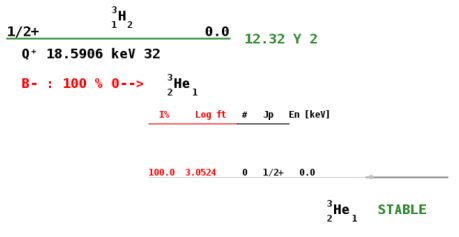
\includegraphics[width=0.47\textwidth]{2Introduction/esquema_niveles_energeticos.png}}
  \subfloat[Graphic representation of tritium decay \cite{TritiumDecayImage}]{
   \label{fig:GraphicDesintegration}
    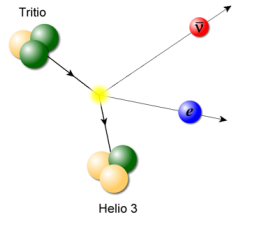
\includegraphics[width=0.53\textwidth]{2Introduction/representacion_desintegracion.png}}
 \caption{Tritium decay}
 \label{fig:TritiumDecay}
\end{figure}

The energy that is released in this nuclear reaccion is constant, $18.6~\keV$, but it is divided between the products of this reaccion. Therefore not all beta particle (electrons) will have the maximum energy. This is what we can see in the figure \ref{fig:TritiumDecaySpectrum}, which is the energetic spectrum of the electrons which are emitted in the tritium decay. The maximum energy of this electrons is $18.6~\keV$ (when beta particles have all the energy), which is the endpoint energy of this spectrum, the average energy is $5.7~\keV$ and the most likely value is slightly below of the average energy, around $4.5~\keV$.

\begin{figure}[hbtp]
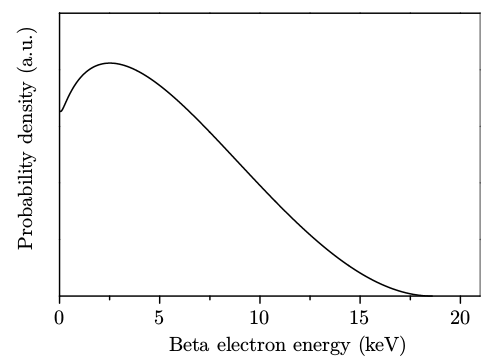
\includegraphics[scale=0.6]{2Introduction/Espectro.png}
\centering
\caption{Energy spectrum of tritium electrons ~\cite{TesisTritio}\label{fig:TritiumDecaySpectrum}}
\end{figure}

Keep in mind that, although the helium isotope is stable, it will be exited immediately after this decay. As a consequence, after the tritium $\beta^-$ decay, we will have a subsequent dexcitation of the $\ce{^{3}He}$ which will produce fotons, $\gamma$, with several well-defined energies that correspond to their energy levels, X-rays. COMPROBAR... It doesn't affect directly to our detector due to the efficiency of our detector at those wavelenghts, as we will se in the chapter \ref{}, section \ref{},  but it could be affect indirectly. BUSCAR ESTAS ENERGÍAS Y VER SI SON TAN DIFERENTES COMO PARA NO AFECTAR DIRECTAMENTE O SE PARENCE A LAS DEL TRITIO Y SI AFECTAN DIRECTAMENTE.

The releasing energy, which is produced in the tritium decay, is very little. In fact, it is the radioactive isotope with the lowest energy released in its $\beta$ disintegration \cite{TritiumHandling}. As a consequence the $\beta$ particles which is emitted in this tritium decay will have a very little mean free path as you can see in the table \ref{MeanFreePathTritium}.

\begin{table}[htbp]
\begin{center}
\begin{tabular}{|c|c|c|}
\hline
Material & Energy ($\beta$)(keV) & Penetration Depth \\
\hline \hline \hline
$\ce{\ce{^{3}_{1}H_2}}$, STP & 5.7 & 0.26 cm \\ \hline
$\ce{\ce{^{3}_{1}H_2}}$, STP & 18.6 & 3.2 cm \\ \hline
Air, STP & 5.7 & 0.036 cm \\ \hline
Air, STP & 18.6 & 0.45 cm \\ \hline
\parbox{10em}{\centering Water, soft tissue\\  (solid matter whose \\  density is $1~\gram\cdot\cm^{-3}$)} & 5.7 & 0.42 $\mu\meter$\\ \hline
\parbox{10em}{\centering Water, soft tissue\\  (solid matter whose \\  density is $1~\gram\cdot\cm^{-3}$)} & 18.6 & 5.2 $\mu\meter$ \\ \hline
\end{tabular}
\caption{Mean Free Path of tritium isotope for several energies~\cite{TritiumHandling}}
\label{MeanFreePathTritium}
\end{center}
\end{table}

On the one hand, it means that the tritium electrons is easily stopped even for simply walls like our clothes, the laboratories gloves or even the our skin it-self, that's, the radioactive hazard is low. Nevertheless, the danger of tritium is increased when tritium is ingested or inhaled because if it has enough radiactivity it can affect to our internal organs because it has a high biologic life time, $9.5$ days \cite{TritiumHandling}, time during which tritium remains in our body and we will be receiving dose due to tritium radiation. Therefore, their health hazard is high.

On the other hand, this short mean free path will be a problem when we try to detect tritium and due to that, there are some limitations which we will have to take into account when we design our detector. 

Tritium has different physical properties than other natural isotopes of the hydrogen like different boilling points as you can see in the table \ref{BoillingPoints} or the property of auto-radiolysis which only happens when radioactive elements are presented. The auto-radiolysis exists because the energy released in tritium decay is larger than the energy bond of oxigen and hydrogen in water molecules ($5.2~\eV$) or the ionization energy of water molecules ($12.6~\eV$) so it can break up these molecules \cite{AutoRadyolisis}. Due to the auto-radiolysis, some radicals appear in the water whose corrosivity is increased.

\begin{table}[htbp]
\begin{center}
\begin{tabular}{|l|l|l|}
\hline
Molecule & Boiling point (for gases) ($\kelvin$) & oxidation form\\
\hline \hline \hline
$\ce{H_2}$ & 20.39 & $\ce{H_2 O}$ \\ \hline
$\ce{HD}$ & 22.14 & $\ce{HDO}$ \\ \hline
$\ce{HT}$ & 22.92 & $\ce{HTO}$ \\ \hline
$\ce{D_2}$ & 23.66 & $\ce{D_2 O}$ \\ \hline
$\ce{DT}$ & 24.38 & $\ce{DTO}$ \\ \hline
$\ce{T_2}$ & 25.04 & $\ce{T_2 O}$ \\ \hline
\end{tabular}
\caption{Gas molecules of hydrogen isotopes and their boiling points}
\label{BoillingPoints}
\end{center}
\end{table}

Although tritium has different physical properties it has almost the same chemical behaviour than other hydrogen isotopes. Tritium, like hydrogen, is a gas at standard conditions of temperature ($273~\kelvin$) and preassure ($1$ atm) forming a two-atom molecules which can be $\ce{HT}$, $\ce{DT}$ and $\ce{T_2}$. It can become in tritium water through oxidation and exchange reactions as you can see in the following chemical ecuations\cite{TritiumHandling}:

\begin{equation}
\begin{split}
& Oxidation: \qquad \qquad \qquad \qquad \qquad \qquad Excahnge\\
& 2\cdot{}\ce{HT} + \ce{O_2} \rightarrow 2 \cdot{} \ce{HTO} ~ \quad \qquad \qquad \qquad \ce{HT} + \ce{H_2 O} \rightarrow \ce{H_2} + \ce{HTO}\\
& 2\cdot{}\ce{T_2} + \ce{O_2} \rightarrow 2 \cdot{} \ce{T_2 O} \qquad \qquad \qquad \qquad \ce{T_2} + \ce{H_2 O} \rightarrow \ce{HT} + \ce{HTO}
\label{OxidationExchange}
\end{split}
\end{equation}

Due to this chemical similarity tritium water can performe the same chemical process than non-radiactive water, some times with higher rate if the tritium concentration is high enough to catalyze the reaction. Its biological hazard comes from this chemical similarity since tritium water is able to substitute normal water in human body. On top of that, tritium water has a higher absorption in human body, around 99\%, than tritium gas, whose absorption in the human body is less than $5 \cdot 10^{-3}\%$  by inalation or practically negligible by skin absorption \cite{TritiumHandling} so it is more dangerous.